
\subsubsection{Claim of Tilt Observer}

\begin{revquote}
The Tilt Observer and its convergence properties are not novel in this work; they originate from prior work ([19]). Where the overall claim is to "This article presents VALINOR (Velocity-Aided Leg Inertial Nonlinear Odometry and Registration), a method for Leg-Inertial odometry for humanoid robots addressing the challenge of lightweight yet accurate and certifiable state estimation.", this could be misleading. It is used as a tool.
\end{revquote}

We thank the reviewer for pointing that out and agree that our formulation was unintentionally ambiguous. The Tilt Observer is indeed not a contribution of this paper itself, since the contribution is its combination with a Leg Odometry, that preserves its accuracy and guarantees. We have therefore fully revised the abstract to eliminate any ambiguity regarding our contributions and claims, and notably state explicitly that {\scshape Valinor} builds upon the Tilt Observer.

\begin{revquote}
The observer dynamics uses a variable $\hat{\boldsymbol{x}}_{2}^{\prime} $, which is not defined in the current paper, despite playing a central role in the update laws.
\end{revquote}

We thank the reviewer for this rightful comment. We have added the definition of $\hat{\boldsymbol{x}}_{2}^{\prime} $ and its role in the filter, right below its use in Eq.~\eqref{eq:tilt_dynamics_1}. We elaborate here the explanation:
The particularity of the Tilt Observer is that it estimates the IMU's tilt $\boldsymbol{x}_{2}$ in two stages. $\hat{\boldsymbol{x}}_{2}^{\prime} $ is its intermediate estimate, which is not constrained to remain on the sphere $\mathbb{S}^{2}$, unlike $\boldsymbol{x}_{2}$ which is a unit vector. As explained in Theorem 1 of~\cite{benallegue2020LyapunovStableOrientationEstimatorHumanoids}, this allows $\hat{\boldsymbol{x}}_{2}^{\prime} $ to converge globally exponentially through the unit sphere. In the second stage of the tilt estimation, the final estimate $\hat{\boldsymbol{x}}_{2}$, is driven by $\hat{\boldsymbol{x}}_{2}^{\prime}$ while being restricted to lie on the unit sphere by the use the formalism of the $\mathbb{S}^{2}$ Lie group. Doing so, the tilt estimate benefits from strong mathematical convergence guarantees while being mathematically consistent.


\begin{revquote}
The observer relies on gains $\alpha_{1}$, $\alpha_{2}$, $\gamma$, but no method or rationale is provided for how they are selected, or tilt observer defines them.
\end{revquote}

We thank the reviewer for this comment. We indeed did not provide a method for the gains tuning. To correct this, we now refer to~\cite{benallegue2023velocity} when introducing the gains in Section~\ref{subsec:tilt_def}. Section IV C of~\cite{benallegue2023velocity} provides insights on how to tune them when working with real systems, notably based on the noisiness and reliability of the IMU and linear velocity measurements:
\begin{quotepaper}
  There are five kinds of gains in this observer, and
while higher gains produce faster convergence, finding
appropriate values for real signals may require some skills.
Here we present the theories and experimental feedback
on how we tend to tune them.
\begin{enumerate}
  \item $\alpha_1$ defines the trust mostly in the measurements yv
of the linear velocity but also in the accelerometer’s
data ya. If these sources are reliable then high
gains will give good performances. If they are not
trustworthy, the observer can still be used since the
estimator will treat these sources through complementary
filtering, but lower gains are recommended.
\item $\alpha_ i  (i \in 2, ..., n)$ defines the intermediate level of
filtering. High values give importance to the linear
velocity estimate $\hat{\boldsymbol{x}}_{1}$ by lowering the related cutoff
frequency of the complementary filter. The gains
would take intermediate values to average between
the gyrometer feedforward and linear-velocity-based
correction, depending on the trust we have in the
corresponding sensor measurements.
\item $\gamma$ or $\rho_1$ defines the final level of filtering of the tilt
estimator, high values give more trust in the firststage
estimation $\hat{\boldsymbol{x}}_{2}^{\prime} $, and lower ones give more trust in
the integration of the gyrometer, producing smoother
outputs.
\item $\rho_2$ defines the trust we have to let the magnetometer
measurements ym influence the tilt estimation.
Therefore, it is usually very low.
\item $\mu$ defines the impact of the magnetometer measurements
ym on the yaw definition. It is tuned similarly
to any nonlinear complementary filter.
\end{enumerate} 

\end{quotepaper}

In our implementation, we used the following tuning: $\alpha_{1} = 4, \alpha_{2} = 4, \gamma = 1$. HRP-5P and RHP Friends are equipped with high-end IMUs\footnote{Unfortunately only the model of the IMU used in HRP5-P (KVH Industries: 1750, according to~\cite{Kaneko2019Hrp5}) has been publicly disclosed.}, so we tuned our filter to leverage them. 
To the paragraph, we also added the note that the convergence properties of the filter are independent of the gains tuning.

\subsubsection{IMU Bias and Noise Modeling}

\begin{revquote}
* IMU measurements (gyroscope and accelerometer) are used directly without modeling or compensating for sensor bias.
* Unlike RI-EKF, which includes IMU bias in the state vector, VALINOR assumes ideal IMU signals.
* This assumption should be acknowledged and tested for robustness, particularly in longer or more dynamic trials.
\end{revquote}

We thank the reviewer for this comment. The biases on the gyrometer and accelerometer measurements were indeed not considered in the Tilt Observer. These biases are one of the core challenges of proprioceptive estimation, since they are not observable with no global position and orientation measurement. In RI-EKF, the authors explain that by simply adding biases to the state, most of their theoretical properties (for example their observability analysis) no longer hold. The complementary filter used for the Tilt Observer is no exception, and adding the biases would prevent from writing a proof of convergence.
But we would like to try and provide more insights on the impact of biases on the estimator, focusing on Eqs.~\eqref{eq:tilt_dynamics_1} and~\eqref{eq:tilt_dynamics_2}. 
The estimator will deviate (but  not diverge) due to the biases. In static, it gives the following static errors:
\begin{align}
  \tilde{\boldsymbol{x}}_{1}&=-\left(\frac{\alpha_{2}}{g_{0}}\boldsymbol{I}+\frac{1}{g_{o}}S\left(\boldsymbol{b}_{g}\right)\left(\alpha_{1}\boldsymbol{I}+S\left(\boldsymbol{b}_{g}\right)\right)\right)^{-1}\left(S\left(\boldsymbol{b}_{g}\right)\boldsymbol{x}_{2}+\frac{1}{g_{o}}S\left(\boldsymbol{b}_{g}\right)\boldsymbol{b}_{a}\right) \\
  \tilde{\boldsymbol{x}}_{2}&=\frac{1}{g_{o}}\left(S\left(\boldsymbol{b}_{g}\right)-\alpha_{1}\boldsymbol{I}\right)\tilde{\boldsymbol{x}}_{1}+\frac{1}{g_{o}}\boldsymbol{b}_{a}
\end{align}
with $\tilde{\boldsymbol{x}}_{1} = \boldsymbol{x}_{1} - \hat{\boldsymbol{x}}_{1}$ and $\tilde{\boldsymbol{x}}_{2} = \boldsymbol{x}_{2} - \hat{\boldsymbol{x}}_{2}$ the errors on the IMU's linear velocity and tilt, respectively. $\boldsymbol{b}_{g}$ and $\boldsymbol{b}_{a}$ the biases on the gyrometer and accelerometer measurements, respectively, and $S\left(\boldsymbol{x}\right)$ the skew-symmetric (cross-product) matrix of the vector $\boldsymbol{x}$. 


To conclude on this response, adding the gyrometer bias to the estimation (which is the most common case, the accelerometer bias is generally not considered in proprioceptive methods) may indeed improve the estimation, but from our experience working with estimators using only proprioceptive measurements, the estimated gyrometer bias generally doesn't converge towards the actual one but to totally unrelated values. It may even reach non-negligible erroneous values that lead to the drift of the robot's estimated state. To give an example, Figure~\ref{fig:bias} below shows the gyrometer bias along the z axis estimated by the RI-EKF during Experiment 1, against an approximation of its actual value at the end of the experiment, obtained by computing the average of the gyrometer measurement over the last 3 seconds while the robot was standing still. We can observe that while the gyrometer bias was low at the end of the walk, the RI-EKF estimated a non-negligible bias, leading to an error of about $5.5 10e^{-4}$ rad/s (so 0.03 deg/s) and to a progressive drift in yaw over time, which can actually be observed in Figure~\ref{fig:traj_friends}.

\begin{figure*}[!ht]
\begin{center}
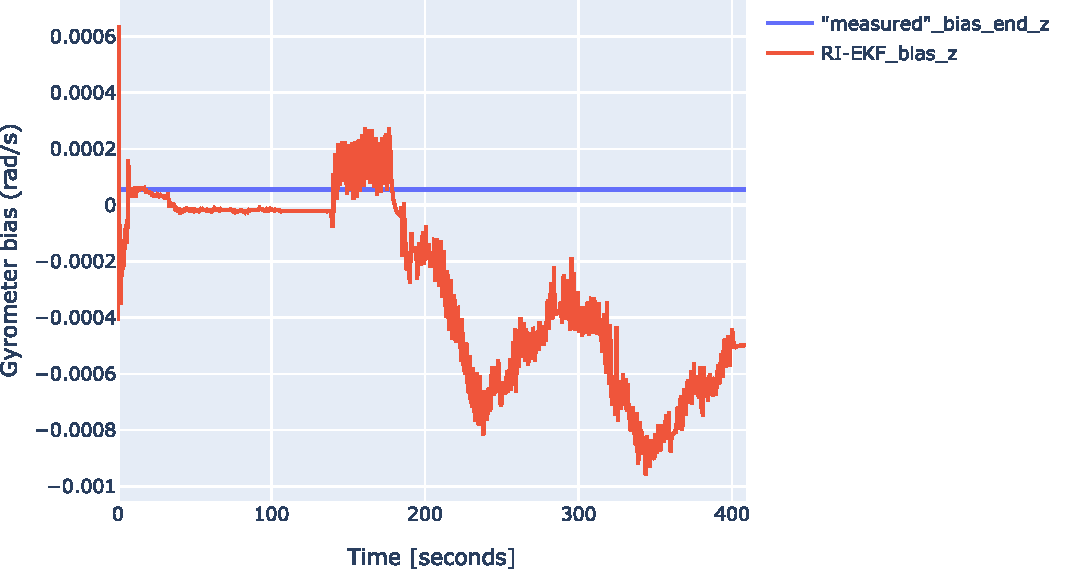
\includegraphics[width=\textwidth]{bias_z.pdf} 
\vskip -0.5pc
\caption{Gyrometer bias along the z axis estimated by the RI-EKF, against its "ground truth".}\label{fig:bias}
\end{center}
\vskip -1.5pc
\end{figure*}

For these reasons, we did not insist on the inclusion of sensor biases, but we have added a discussion on this point to the conclusion of the revised version.


 

\subsubsection{End-to-End Pipeline and Description}




\begin{revquote}\hypertarget{CommentSe3Fusion}{}
There is no formal SE(3), Lie group, or EKF-based structure defined for global pose fusion.
\end{revquote}


We thank the reviewer for this comment. The proposed estimator indeed doesn't use an EKF or the Lie Group SE(3) to perform fusion, but builds a pose from a position, a yaw, and a tilt coming from different sources (from contact positions, contact orientations, and the Tilt Observer, respectively). Our main contribution in terms of fusion is the axis-agnostic fusion, which in addition to being mathematically sound, allows to preserve the Tilt Observer's tilt estimate during the fusion with the Leg odometry's yaw, and thus its accuracy and convergence guarantees. We agree that this can probably be improved, as we recognized in the conclusion of the initial submission of the paper. However, fusing the variables coming from the different sources while keeping the philosophy of lightweight yet reliable estimation is not trivial. 
As an example, we could indeed fuse the contact poses and the output of the Tilt Observer within an EKF. However, the matrix inversion and multiplications involved in the EKF would increase the computation time of our estimator. Moreover, by using our tilt estimate $\hat{\boldsymbol{x}}_{2}$ as a measurement within the EKF, we could not guarantee anymore the convergence properties of the tilt at the output.

To remain consistent with our approach, we are thus working on extending our method by writing a proof of convergence similar to that of the Tilt Observer, for a complementary filter that would include the positions and orientations coming from contacts. 




\begin{revquote}
- While experimental sections reference a combined system (estimator + control + humanoid), there is no detailed diagram or explanation of the full data flow. Pose estimation is described in parts (e.g., contact anchoring, tilt fusion), but the overall architecture is fragmented and unclear.
\end{revquote}


We thank the reviewer for these comments. We agree that the overall architecture of our estimate can be unclear. To clarify it, we added Figure~\ref{fig:summary} at the beginning of the paper, a block diagram which provides an overview of the whole framework and the contribution of each block and section. We think this will enhance the readability of the paper.

\begin{revquote}
Though contact positions relative to the IMU are derived from encoder data, the process of estimating the anchor pose, its reference frame, and how it updates over time is not fully described.
\end{revquote}

We thank the reviewer for this comment. The anchor point is a point that belongs to the robot, but we consider its position and velocity in both the world and the IMU's frame. By assuming this point has a zero linear velocity in the world, we can obtain an estimate of the IMU's velocity in the world with Eq.~\eqref{eq:yv}. To compute this velocity, we don't need to compute the position and linear velocity of the anchor point in the world frame, but only its position and linear velocity in the IMU's frame. The latter can be computed directly from the position and linear velocity of contacts in the IMU (thus using encoder data) using Eq.~\eqref{eq:imuAnchorKine}. 
We revised Section~\ref{sec:anchor_point} to improve the flow of this explanation of the computation of the anchor point kinematics, in order to make it clearer. We now also explicit the fact we compute ${^{\mathcal{I}}}\boldsymbol{p}_{\mathcal{A}}$ and ${^{\mathcal{I}}} \dot{\boldsymbol{p}}_{\mathcal{A}}$ using Eq.~\eqref{eq:imuAnchorKine} on each iteration, and that they are the ones that will be used later to compute Eq.~\eqref{eq:yv}:
\begin{quote}
  ``${^{\mathcal{I}}}\boldsymbol{p}_{\mathcal{A}}$ and ${^{\mathcal{I}}} \dot{\boldsymbol{p}}_{\mathcal{A}}$ are updated at each iteration. As explained in Section~\ref{subsec:tiltMeas}, by combining them with the zero-velocity assumption of the anchor point in the world frame and the gyrometer measurement, we obtain an algebraic estimate of the IMU velocity in the world frame.''
\end{quote}

 

\subsubsection{Quantitative Yaw Visualization}

\begin{revquote}
Yaw fusion is one of the core contributions of the paper (via the axis-agnostic method), yet no plot of yaw angle or yaw error over time is provided. This significantly weakens the experimental validation of the claimed improvement.
\end{revquote}

We thank the reviewer for this comment. The yaw estimation is indeed important in proprioceptive odometry, so we include its plot over time to Figure~\ref{fig:pose_rhps1}.

However, we would like to highlight that our contribution here is a novel method for the fusion of a yaw and a tilt estimates coming from different sources, but not an improvement of yaw estimation by proprioceptive methods. In the proposed estimator, the yaw estimate comes solely from Leg odometry, it is therefore not expected to be more accurate than the yaw estimated by the RI-EKF, which also leverages the IMU measurements. As elaborated in \hyperlink{CommentSe3Fusion}{response to Comment 5}, combining Leg odometry and IMU measurements in our framework is not trivial, but we are currently addressing it.

The fusion we propose here allows us to construct an orientation matrix from the tilt coming from the Tilt Observer, and the yaw coming from the Leg odometry.
This fusion is important here since it allows to preserve the mathematical convergence guarantees provided by the Tilt Observer within our full orientation, in addition to being robust to singularities. 
We have noticed that we did not insists on this enough in the paper, so we clarified it in our Abstract, Section~\ref{sec:leg_odometry}, and Section~\ref{sec:axisAgnostic}, which explain the leg odometry and the axis-agnostic fusion, respectively.



\begin{revquote}
In Figure 5, VALINOR exhibits larger variations in vertical translation (z-axis) compared to RI-EKF. This raises concerns that the improved orientation or tilt accuracy may come at the cost of position accuracy, particularly in vertical drift.
\end{revquote}

We thank the reviewer for this comment. You are right pointing out that we indeed drift slightly faster along the z axis than the RI-EKF.
However, this drift is not due to the tilt estimate, which we believe it is beneficial to our odometry. 
This drift is actually due to a problem inherent to Leg odometry, which highly relies on the contact detection timing. When detecting a contact too early or too late, the robot's internal flexibilities will lead to errors in the forward kinematics from the IMU to the contact, and thus to a discrepancy in the pose estimate, notably along the z axis. If this detection issue is repeatable, this induces a drift, incremented at each step, as we observe here.
The RI-EKF is also affected by this drift, but it is slightly corrected by the IMU measurements it leverages. Also, the RI-EKF appends feet positions to their state vector, allowing to correct them slightly over time. In our experiment, contacts are detected using a simple Schmitt trigger on the force measured at the contact. By tuning the Schmitt trigger's thresholds, we can indeed reduce the drift along the z axis, and thus improve our odometry results. However, we decided to leave them unchanged for fairness in the comparison. 


What's more, you can notice that the height estimated by the RI-EKF suddenly plunges at around 10s, to then suddenly increase at around 50s. Since we already used the RI-EKF as a comparison with a previous work (“The Kinetics Observer: A Tightly Coupled Estimator for Legged Robots,” preprint, 2024), on the same dataset, we already noticed this behavior, and explained it by the erroneous estimate of the robot's pitch angle by the RI-EKF at that time:

\begin{quotepaper}
`` ... we see that at about 10 seconds after
the start, the RI-EKF’s estimate of this position suddenly and
erroneously decreased, to then increase greatly at about 50
seconds after the start. We verify that this translation error is
mainly due to a misestimation of the pitch angle. Between
10 seconds and 50 seconds, the robot walked 7.2 meters and
the average error on the pitch estimated by the RI-EKF was
1.5◦. The resulting error in elevation $\Delta z = tan(1.5) \times 7.2$
would be about 19 cm, which roughly corresponds to the drift we can see ...''
\end{quotepaper}

What's more, we could observe this behaviour on each of the five trials of this walk experiment (Experiment 1), while our tilt estimate has been consistently relatively accurate throughout all experiments, as shown by its low standard deviation overall.
This is to our point of view a critical issue, that counterbalances the RI-EKS's slower drift, but we did not want to insist on it for fairness. 
Since both estimators have strengths and weaknesses in vertical translation estimation, we did not declare one superior in our evaluation. However, we modified the conclusion of Section~\ref{subsec:est_accur_eval} to provide an explanation on the observed drift by both estimators, and discuss this point. We have also added to~\ref{sec:exps} the criteria an estimator should meet to be used in our intended use case, namely, providing feedback for remote control or task planning and execution in the robot's local workspace. Doing so, we clarify from the beginning that the absolute drift in position and yaw is anyway not the most relevant metric for proprioceptive odometry evaluation because of its lower determinism by such methods. 



To conclude, we think the robustness and accuracy provided by our reliable tilt estimate is a strength that can be exploited to improve proprioceptive odometry further. We are confident that our method still has considerable room for improvement, which would notably come from leveraging IMU measurements in the position and yaw estimations. As explained in (\hyperlink{CommentSe3Fusion}{response to Comment 5}), we are working on the direct combination of the Tilt Observer and Leg odometry within a single complementary filter. We are also exploring ways to correct the contact reference poses over time, as performed by the RI-EKF.



\subsubsection{Experimental Coverage}

\begin{revquote}
The proposed estimator appears to be an advanced method with efficiency and modularity benefits. It would be reasonable to expect greater generalization across various robot behaviors and environments.
However, the current experiments are confined to flat, short-range, structured lab environment, which limits the real-world relevance of the evaluation.
The test conditions can benefit from:
    o Uneven or non-planar surfaces
    o Inclines or stairs
    o Long-distance walking (to test drift)
\end{revquote}

We thank the reviewer for this comment and for believing in our work. We are indeed convinced that our methods can be useful thanks to its computational efficiency and accuracy.
However, your comment made us realize we should make clearer that our estimator is well suited for some use cases, for example for providing feedback for remote control or task planning and execution in the robot's local workspace, but not for any situtation. We now precise our targeted use cases from the beginning of~\ref{sec:exps} and in the abstract of the revised paper, and clarify our claims in the Conclusion, notably explaining that in use cases where a minimal absolute drift in the pose is required, other methods like ones using exteroceptive measurements would still be more appropriate. If you are interested, we elaborated on the expected behaviour of our method in more difficult situations in response to \hyperlink{Comment 2 Rev 3}{Comment 2 by Reviewer 3}.


Proprioceptive odometry is bounded to drift over time and cannot recover the global pose after failure. For example, if the yaw were to drift up to a -180 degree error, the translation would be estimated in the opposite direction to the actual one. It has thus been commonly acknowledged that the most relevant way to evaluate it is not by computing the estimation error over long distances, but by computing statistical errors over shorter distances with the Relative Error (e.g. "Legged robot state estimation with invariant extended kalman filter using neural measurement network.", by Youm, Donghoon, et al., ~\cite{yoon2023InvariantSmootherDynamicContactEventInformation}). We thus computed the Relative Error over 1 meter for Experiment 1 (walk on flat ground) and over 0.3 meters for Experiment 2 (multi-contact motion on tilted obstacles). Therefore, in total, the Relative Error was computed over about:
\begin{itemize}
    \item 90 independent sub-trajectories for the 'Odometry on Flat Ground' experiment (90 meters in total).
    \item 26 independent sub-trajectories for the 'Multi-contact Motion with Tilted Obstacles' experiment (8 meters in total).
\end{itemize}
To increase the relevance of our results, we performed our experiments on two different robots and conducted every experiments in a motion capture environment, since precision over short translations matters the most. Experiment 2 involved contacts on both legs and on the left hand, at different heights and inclinations, in order to prove the adaptability of our estimator to non-flat environment.



\subsubsection{Computation Time Analysis}

\begin{revquote}
The core runtime claim is strong:
      o VALINOR = 2.547 µs
      o RI-EKF = 19.315 µs
However, this leads to some open questions as
      o Is the timing consistent across all trials?
      o How does performance vary with the number of contacts?
    
\end{revquote}

We thank the reviewer for this comment and these very relevant questions. The provided 2.547 µs is an average between the mean computation times obtained throughout the four trials of Experiment 2 (multi-contact motion), which involved 3 contacts. In the table below, are regrouped the mean computation times by each estimator, obtained for each sequence, the standard deviation between them, and their average. As you can see through the very low standard deviation, both estimators have consistent computation times accross all sequences. 
Building on your comment, we have added this standard deviation to our results to prove the consistency of our method.

\begin{table}[!h]
  \begin{center}
        \begin{tabu}to\linewidth{| X[c] | X[c] | X[c] | X[c] | X[c] | X[c] | X[c] | }
            \hline
              & Trial 1 & Trial 2 & Trial 3 & Trial 4 & Mean & Std \\
            \hline
             Valinor & 2.579 $\mu s$  & 2.567 $\mu s$  & 2.457 $\mu s$  & 2.556 $\mu s$  & 2.547 $\mu s$ & 0.043 $\mu s$ \\
             \hline 
             Hartley & 20.268 $\mu s$ & 18.642 $\mu s$ & 19.197 $\mu s$ & 19.154 $\mu s$ & 19.315 $\mu s$ & 0.529 $\mu s$ \\
            \hline     
        \end{tabu}
    \end{center}
\end{table}

Our method scales very well with respect to the number of contacts, since an additional contact only implies:
\begin{itemize}
  \item An additional computation of Eq.~\eqref{eq:ratio_ui}, hence negligible operations with floats.
  \item Two additional sums of 3x1 vectors in Eq.~\eqref{eq:imuAnchorKine}.
  \item The orientation average in Eq.~\eqref{eq:leg_odom_avg_ori} is computed between the two most reliable contacts, so over 2 contacts, no additional operation is involved. 
  \item An additional product of a 3x1 vector by a 3x3 matrix and the difference between two 3x1 vectors in Eq.~\eqref{eq:est_p_imu}.
\end{itemize}

These operations, in addition to being extremely fast, scale at most linearly with the number of contacts.


In comparison, the RI-EKF, due to the matrix multiplications and inversion, would scale at least quadratically with the number of contacts.

